\section{Projektarbeit Evaluation}

\begin{frame}{Rückblick}
	\begin{columns}
		\begin{column}{0.5\textwidth}
			Projektarbeit MANVSim 
			\begin{itemize}
				\item Weekly Termin mit ergänzenden Einzelterminen
				\item Feature-Branch Implementierung
				\item Review Prozesse für gemeinsamen Wissensaustausch
			\end{itemize}
			Herausforderungen
			\begin{itemize}
				\item Unterschiedliches KnowHow vereinen
				\item Mehrere Entwicklungsschwerpunkte (Web, Python, Mobile)
				\item Stundenpläne und (Krank-)Ausfälle ändern Prioritäten
			\end{itemize}
		\end{column}
		\begin{column}{0.5\textwidth}
			\centering
			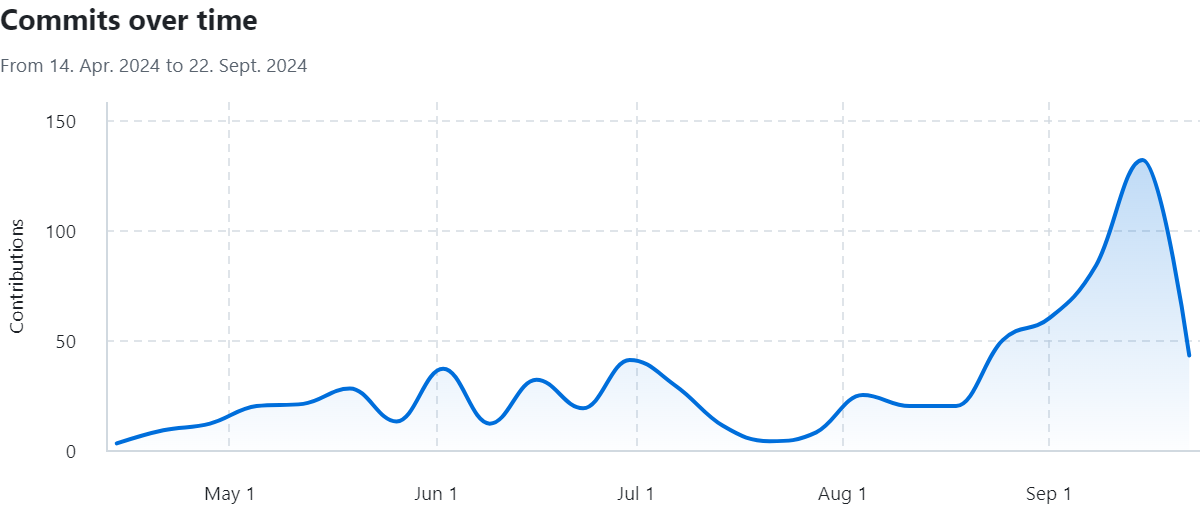
\includegraphics[height=0.4\textheight]{images/Commits_over_time.png}
		\end{column}
	\end{columns}
\end{frame}
\begin{frame}{Ausblick}
	Future Work - Webanwendung
	\begin{itemize}
		\item Erweiterung/Optimieren der Admin-Oberflächen
		\item Neustarten von Übungen basierend auf LogEvents
		\item Statistische Auswertung
		\item User-Management Komponente + Rollen/Rechte erweitern 	
	\end{itemize}

    Future Work - Mobile App / GameAPI
	\begin{itemize}
		\item Resourcen in Inventar Management integrieren
		\item Verbessertes Monitoring der Teilnehmer
		\item Teilnehmer über Hinweise anleiten
		\item IOS Deployment optimieren
	\end{itemize}
\end{frame}